\documentclass[1p]{elsarticle_modified}
%\bibliographystyle{elsarticle-num}

%\usepackage[colorlinks]{hyperref}
%\usepackage{abbrmath_seonhwa} %\Abb, \Ascr, \Acal ,\Abf, \Afrak
\usepackage{amsfonts}
\usepackage{amssymb}
\usepackage{amsmath}
\usepackage{amsthm}
\usepackage{scalefnt}
\usepackage{amsbsy}
\usepackage{kotex}
\usepackage{caption}
\usepackage{subfig}
\usepackage{color}
\usepackage{graphicx}
\usepackage{xcolor} %% white, black, red, green, blue, cyan, magenta, yellow
\usepackage{float}
\usepackage{setspace}
\usepackage{hyperref}

\usepackage{tikz}
\usetikzlibrary{arrows}

\usepackage{multirow}
\usepackage{array} % fixed length table
\usepackage{hhline}

%%%%%%%%%%%%%%%%%%%%%
\makeatletter
\renewcommand*\env@matrix[1][\arraystretch]{%
	\edef\arraystretch{#1}%
	\hskip -\arraycolsep
	\let\@ifnextchar\new@ifnextchar
	\array{*\c@MaxMatrixCols c}}
\makeatother %https://tex.stackexchange.com/questions/14071/how-can-i-increase-the-line-spacing-in-a-matrix
%%%%%%%%%%%%%%%

\usepackage[normalem]{ulem}

\newcommand{\msout}[1]{\ifmmode\text{\sout{\ensuremath{#1}}}\else\sout{#1}\fi}
%SOURCE: \msout is \stkout macro in https://tex.stackexchange.com/questions/20609/strikeout-in-math-mode

\newcommand{\cancel}[1]{
	\ifmmode
	{\color{red}\msout{#1}}
	\else
	{\color{red}\sout{#1}}
	\fi
}

\newcommand{\add}[1]{
	{\color{blue}\uwave{#1}}
}

\newcommand{\replace}[2]{
	\ifmmode
	{\color{red}\msout{#1}}{\color{blue}\uwave{#2}}
	\else
	{\color{red}\sout{#1}}{\color{blue}\uwave{#2}}
	\fi
}

\newcommand{\Sol}{\mathcal{S}} %segment
\newcommand{\D}{D} %diagram
\newcommand{\A}{\mathcal{A}} %arc


%%%%%%%%%%%%%%%%%%%%%%%%%%%%%5 test

\def\sl{\operatorname{\textup{SL}}(2,\Cbb)}
\def\psl{\operatorname{\textup{PSL}}(2,\Cbb)}
\def\quan{\mkern 1mu \triangleright \mkern 1mu}

\theoremstyle{definition}
\newtheorem{thm}{Theorem}[section]
\newtheorem{prop}[thm]{Proposition}
\newtheorem{lem}[thm]{Lemma}
\newtheorem{ques}[thm]{Question}
\newtheorem{cor}[thm]{Corollary}
\newtheorem{defn}[thm]{Definition}
\newtheorem{exam}[thm]{Example}
\newtheorem{rmk}[thm]{Remark}
\newtheorem{alg}[thm]{Algorithm}

\newcommand{\I}{\sqrt{-1}}
\begin{document}

%\begin{frontmatter}
%
%\title{Boundary parabolic representations of knots up to 8 crossings}
%
%%% Group authors per affiliation:
%\author{Yunhi Cho} 
%\address{Department of Mathematics, University of Seoul, Seoul, Korea}
%\ead{yhcho@uos.ac.kr}
%
%
%\author{Seonhwa Kim} %\fnref{s_kim}}
%\address{Center for Geometry and Physics, Institute for Basic Science, Pohang, 37673, Korea}
%\ead{ryeona17@ibs.re.kr}
%
%\author{Hyuk Kim}
%\address{Department of Mathematical Sciences, Seoul National University, Seoul 08826, Korea}
%\ead{hyukkim@snu.ac.kr}
%
%\author{Seokbeom Yoon}
%\address{Department of Mathematical Sciences, Seoul National University, Seoul, 08826,  Korea}
%\ead{sbyoon15@snu.ac.kr}
%
%\begin{abstract}
%We find all boundary parabolic representation of knots up to 8 crossings.
%
%\end{abstract}
%\begin{keyword}
%    \MSC[2010] 57M25 
%\end{keyword}
%
%\end{frontmatter}

%\linenumbers
%\tableofcontents
%
\newcommand\colored[1]{\textcolor{white}{\rule[-0.35ex]{0.8em}{1.4ex}}\kern-0.8em\color{red} #1}%
%\newcommand\colored[1]{\textcolor{white}{ #1}\kern-2.17ex	\textcolor{white}{ #1}\kern-1.81ex	\textcolor{white}{ #1}\kern-2.15ex\color{red}#1	}

{\Large $\underline{12a_{1148}~(K12a_{1148})}$}

\setlength{\tabcolsep}{10pt}
\renewcommand{\arraystretch}{1.6}
\vspace{1cm}\begin{tabular}{m{100pt}>{\centering\arraybackslash}m{274pt}}
\multirow{5}{120pt}{
	\centering
	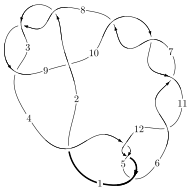
\includegraphics[width=112pt]{../../../GIT/diagram.site/Diagrams/png/1949_12a_1148.png}\\
\ \ \ A knot diagram\footnotemark}&
\allowdisplaybreaks
\textbf{Linearized knot diagam} \\
\cline{2-2}
 &
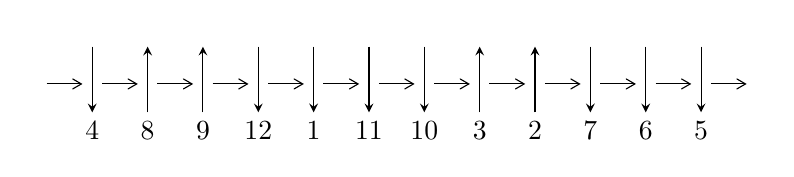
\begin{tikzpicture}[x=20pt, y=17pt]
	% nodes
	\node (C0) at (0, 0) {};
	\node (C1) at (1, 0) {};
	\node (C1U) at (1, +1) {};
	\node (C1D) at (1, -1) {4};

	\node (C2) at (2, 0) {};
	\node (C2U) at (2, +1) {};
	\node (C2D) at (2, -1) {8};

	\node (C3) at (3, 0) {};
	\node (C3U) at (3, +1) {};
	\node (C3D) at (3, -1) {9};

	\node (C4) at (4, 0) {};
	\node (C4U) at (4, +1) {};
	\node (C4D) at (4, -1) {12};

	\node (C5) at (5, 0) {};
	\node (C5U) at (5, +1) {};
	\node (C5D) at (5, -1) {1};

	\node (C6) at (6, 0) {};
	\node (C6U) at (6, +1) {};
	\node (C6D) at (6, -1) {11};

	\node (C7) at (7, 0) {};
	\node (C7U) at (7, +1) {};
	\node (C7D) at (7, -1) {10};

	\node (C8) at (8, 0) {};
	\node (C8U) at (8, +1) {};
	\node (C8D) at (8, -1) {3};

	\node (C9) at (9, 0) {};
	\node (C9U) at (9, +1) {};
	\node (C9D) at (9, -1) {2};

	\node (C10) at (10, 0) {};
	\node (C10U) at (10, +1) {};
	\node (C10D) at (10, -1) {7};

	\node (C11) at (11, 0) {};
	\node (C11U) at (11, +1) {};
	\node (C11D) at (11, -1) {6};

	\node (C12) at (12, 0) {};
	\node (C12U) at (12, +1) {};
	\node (C12D) at (12, -1) {5};
	\node (C13) at (13, 0) {};

	% arrows
	\draw[->,>={angle 60}]
	(C0) edge (C1) (C1) edge (C2) (C2) edge (C3) (C3) edge (C4) (C4) edge (C5) (C5) edge (C6) (C6) edge (C7) (C7) edge (C8) (C8) edge (C9) (C9) edge (C10) (C10) edge (C11) (C11) edge (C12) (C12) edge (C13) ;	\draw[->,>=stealth]
	(C1U) edge (C1D) (C2D) edge (C2U) (C3D) edge (C3U) (C4U) edge (C4D) (C5U) edge (C5D) (C6U) edge (C6D) (C7U) edge (C7D) (C8D) edge (C8U) (C9D) edge (C9U) (C10U) edge (C10D) (C11U) edge (C11D) (C12U) edge (C12D) ;
	\end{tikzpicture} \\
\hhline{~~} \\& 
\textbf{Solving Sequence} \\ \cline{2-2} 
 &
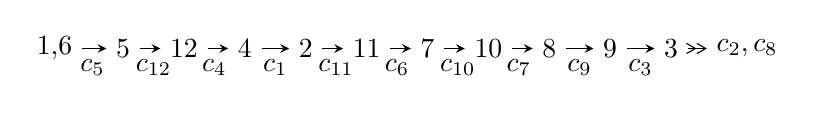
\begin{tikzpicture}[x=22pt, y=7pt]
	% node
	\node (A0) at (-1/8, 0) {1,6};
	\node (A1) at (1, 0) {5};
	\node (A2) at (2, 0) {12};
	\node (A3) at (3, 0) {4};
	\node (A4) at (4, 0) {2};
	\node (A5) at (5, 0) {11};
	\node (A6) at (6, 0) {7};
	\node (A7) at (7, 0) {10};
	\node (A8) at (8, 0) {8};
	\node (A9) at (9, 0) {9};
	\node (A10) at (10, 0) {3};
	\node (C1) at (1/2, -1) {$c_{5}$};
	\node (C2) at (3/2, -1) {$c_{12}$};
	\node (C3) at (5/2, -1) {$c_{4}$};
	\node (C4) at (7/2, -1) {$c_{1}$};
	\node (C5) at (9/2, -1) {$c_{11}$};
	\node (C6) at (11/2, -1) {$c_{6}$};
	\node (C7) at (13/2, -1) {$c_{10}$};
	\node (C8) at (15/2, -1) {$c_{7}$};
	\node (C9) at (17/2, -1) {$c_{9}$};
	\node (C10) at (19/2, -1) {$c_{3}$};
	\node (A11) at (45/4, 0) {$c_{2},c_{8}$};

	% edge
	\draw[->,>=stealth]	
	(A0) edge (A1) (A1) edge (A2) (A2) edge (A3) (A3) edge (A4) (A4) edge (A5) (A5) edge (A6) (A6) edge (A7) (A7) edge (A8) (A8) edge (A9) (A9) edge (A10) ;
	\draw[->>,>={angle 60}]	
	(A10) edge (A11);
\end{tikzpicture} \\ 

\end{tabular} \\

\footnotetext{
The image of knot diagram is generated by the software ``\textbf{Draw programme}" developed by Andrew Bartholomew(\url{http://www.layer8.co.uk/maths/draw/index.htm\#Running-draw}), where we modified some parts for our purpose(\url{https://github.com/CATsTAILs/LinksPainter}).
}\phantom \\ \newline 
\centering \textbf{Ideals for irreducible components\footnotemark of $X_{\text{par}}$} 
 
\begin{align*}
I^u_{1}&=\langle 
u^{36}+u^{35}+\cdots+3 u^2+1\rangle \\
\\
\end{align*}
\raggedright * 1 irreducible components of $\dim_{\mathbb{C}}=0$, with total 36 representations.\\
\footnotetext{All coefficients of polynomials are rational numbers. But the coefficients are sometimes approximated in decimal forms when there is not enough margin.}
\newpage
\renewcommand{\arraystretch}{1}
\centering \section*{I. $I^u_{1}= \langle u^{36}+u^{35}+\cdots+3 u^2+1 \rangle$}
\flushleft \textbf{(i) Arc colorings}\\
\begin{tabular}{m{7pt} m{180pt} m{7pt} m{180pt} }
\flushright $a_{1}=$&$\begin{pmatrix}0\\u\end{pmatrix}$ \\
\flushright $a_{6}=$&$\begin{pmatrix}1\\0\end{pmatrix}$ \\
\flushright $a_{5}=$&$\begin{pmatrix}1\\- u^2\end{pmatrix}$ \\
\flushright $a_{12}=$&$\begin{pmatrix}u\\- u^3+u\end{pmatrix}$ \\
\flushright $a_{4}=$&$\begin{pmatrix}- u^2+1\\u^4-2 u^2\end{pmatrix}$ \\
\flushright $a_{2}=$&$\begin{pmatrix}- u^5+2 u^3- u\\u^7-3 u^5+2 u^3+u\end{pmatrix}$ \\
\flushright $a_{11}=$&$\begin{pmatrix}- u^3+2 u\\- u^3+u\end{pmatrix}$ \\
\flushright $a_{7}=$&$\begin{pmatrix}u^6-3 u^4+2 u^2+1\\u^6-2 u^4+u^2\end{pmatrix}$ \\
\flushright $a_{10}=$&$\begin{pmatrix}- u^9+4 u^7-5 u^5+3 u\\- u^9+3 u^7-3 u^5+u\end{pmatrix}$ \\
\flushright $a_{8}=$&$\begin{pmatrix}u^{12}-5 u^{10}+9 u^8-4 u^6-6 u^4+5 u^2+1\\u^{12}-4 u^{10}+6 u^8-2 u^6-3 u^4+2 u^2\end{pmatrix}$ \\
\flushright $a_{9}=$&$\begin{pmatrix}u^{21}-8 u^{19}+\cdots-4 u^3+3 u\\- u^{23}+9 u^{21}+\cdots+4 u^3+u\end{pmatrix}$ \\
\flushright $a_{3}=$&$\begin{pmatrix}u^{31}-12 u^{29}+\cdots+32 u^5+16 u^3\\u^{31}-11 u^{29}+\cdots+4 u^3+u\end{pmatrix}$\\&\end{tabular}
\flushleft \textbf{(ii) Obstruction class $= -1$}\\~\\
\flushleft \textbf{(iii) Cusp Shapes $= 4 u^{33}-48 u^{31}+4 u^{30}+260 u^{29}-44 u^{28}-804 u^{27}+216 u^{26}+1444 u^{25}-592 u^{24}-1136 u^{23}+892 u^{22}-948 u^{21}-420 u^{20}+3268 u^{19}-948 u^{18}-2672 u^{17}+1812 u^{16}-804 u^{15}-808 u^{14}+2816 u^{13}-896 u^{12}-1200 u^{11}+1080 u^{10}-816 u^9-56 u^8+680 u^7-352 u^6+80 u^5+64 u^4-112 u^3+48 u^2-12 u+2$}\\~\\
\newpage\renewcommand{\arraystretch}{1}
\flushleft \textbf{(iv) u-Polynomials at the component}\newline \\
\begin{tabular}{m{50pt}|m{274pt}}
Crossings & \hspace{64pt}u-Polynomials at each crossing \\
\hline $$\begin{aligned}c_{1},c_{6},c_{7}\\c_{10},c_{11}\end{aligned}$$&$\begin{aligned}
&u^{36}-3 u^{35}+\cdots-12 u+1
\end{aligned}$\\
\hline $$\begin{aligned}c_{2},c_{3},c_{8}\end{aligned}$$&$\begin{aligned}
&u^{36}- u^{35}+\cdots+3 u^2+1
\end{aligned}$\\
\hline $$\begin{aligned}c_{4},c_{5},c_{12}\end{aligned}$$&$\begin{aligned}
&u^{36}+u^{35}+\cdots+3 u^2+1
\end{aligned}$\\
\hline $$\begin{aligned}c_{9}\end{aligned}$$&$\begin{aligned}
&u^{36}+3 u^{35}+\cdots-106 u-187
\end{aligned}$\\
\hline
\end{tabular}\\~\\
\newpage\renewcommand{\arraystretch}{1}
\flushleft \textbf{(v) Riley Polynomials at the component}\newline \\
\begin{tabular}{m{50pt}|m{274pt}}
Crossings & \hspace{64pt}Riley Polynomials at each crossing \\
\hline $$\begin{aligned}c_{1},c_{6},c_{7}\\c_{10},c_{11}\end{aligned}$$&$\begin{aligned}
&y^{36}+49 y^{35}+\cdots-54 y+1
\end{aligned}$\\
\hline $$\begin{aligned}c_{2},c_{3},c_{8}\end{aligned}$$&$\begin{aligned}
&y^{36}-35 y^{35}+\cdots+6 y+1
\end{aligned}$\\
\hline $$\begin{aligned}c_{4},c_{5},c_{12}\end{aligned}$$&$\begin{aligned}
&y^{36}-27 y^{35}+\cdots+6 y+1
\end{aligned}$\\
\hline $$\begin{aligned}c_{9}\end{aligned}$$&$\begin{aligned}
&y^{36}-23 y^{35}+\cdots-458166 y+34969
\end{aligned}$\\
\hline
\end{tabular}\\~\\
\newpage\flushleft \textbf{(vi) Complex Volumes and Cusp Shapes}
$$\begin{array}{c|c|c}  
\text{Solutions to }I^u_{1}& \I (\text{vol} + \sqrt{-1}CS) & \text{Cusp shape}\\
 \hline 
\begin{aligned}
u &= \phantom{-}0.015238 + 0.941216 I\end{aligned}
 & -18.6813 - 5.7665 I & \phantom{-}5.67878 + 2.82103 I \\ \hline\begin{aligned}
u &= \phantom{-}0.015238 - 0.941216 I\end{aligned}
 & -18.6813 + 5.7665 I & \phantom{-}5.67878 - 2.82103 I \\ \hline\begin{aligned}
u &= -0.006373 + 0.933067 I\end{aligned}
 & \phantom{-}14.2459 + 2.3310 I & \phantom{-}2.48067 - 2.82015 I \\ \hline\begin{aligned}
u &= -0.006373 - 0.933067 I\end{aligned}
 & \phantom{-}14.2459 - 2.3310 I & \phantom{-}2.48067 + 2.82015 I \\ \hline\begin{aligned}
u &= \phantom{-}0.922444\phantom{ +0.000000I}\end{aligned}
 & \phantom{-}3.24298\phantom{ +0.000000I} & \phantom{-}1.81830\phantom{ +0.000000I} \\ \hline\begin{aligned}
u &= -1.15188\phantom{ +0.000000I}\end{aligned}
 & -2.33631\phantom{ +0.000000I} & -1.84880\phantom{ +0.000000I} \\ \hline\begin{aligned}
u &= \phantom{-}1.159790 + 0.356655 I\end{aligned}
 & \phantom{-}6.79135 + 0.54642 I & \phantom{-}2.47249 + 0.25591 I \\ \hline\begin{aligned}
u &= \phantom{-}1.159790 - 0.356655 I\end{aligned}
 & \phantom{-}6.79135 - 0.54642 I & \phantom{-}2.47249 - 0.25591 I \\ \hline\begin{aligned}
u &= -1.189470 + 0.302752 I\end{aligned}
 & \phantom{-}0.62502 + 1.83607 I & -1.241747 - 0.124519 I \\ \hline\begin{aligned}
u &= -1.189470 - 0.302752 I\end{aligned}
 & \phantom{-}0.62502 - 1.83607 I & -1.241747 + 0.124519 I \\ \hline\begin{aligned}
u &= \phantom{-}0.076636 + 0.760003 I\end{aligned}
 & \phantom{-}10.05780 - 4.59251 I & \phantom{-}5.76656 + 3.95694 I \\ \hline\begin{aligned}
u &= \phantom{-}0.076636 - 0.760003 I\end{aligned}
 & \phantom{-}10.05780 + 4.59251 I & \phantom{-}5.76656 - 3.95694 I \\ \hline\begin{aligned}
u &= \phantom{-}1.243450 + 0.096073 I\end{aligned}
 & -4.28530 - 2.08913 I & -10.75982 + 5.46611 I \\ \hline\begin{aligned}
u &= \phantom{-}1.243450 - 0.096073 I\end{aligned}
 & -4.28530 + 2.08913 I & -10.75982 - 5.46611 I \\ \hline\begin{aligned}
u &= -1.26918\phantom{ +0.000000I}\end{aligned}
 & -1.54627\phantom{ +0.000000I} & -6.99460\phantom{ +0.000000I} \\ \hline\begin{aligned}
u &= -1.270690 + 0.154646 I\end{aligned}
 & \phantom{-}0.15355 + 4.66558 I & -3.82180 - 6.53875 I \\ \hline\begin{aligned}
u &= -1.270690 - 0.154646 I\end{aligned}
 & \phantom{-}0.15355 - 4.66558 I & -3.82180 + 6.53875 I \\ \hline\begin{aligned}
u &= \phantom{-}1.247480 + 0.302288 I\end{aligned}
 & \phantom{-}0.14493 - 5.48066 I & -3.17694 + 7.52248 I \\ \hline\begin{aligned}
u &= \phantom{-}1.247480 - 0.302288 I\end{aligned}
 & \phantom{-}0.14493 + 5.48066 I & -3.17694 - 7.52248 I \\ \hline\begin{aligned}
u &= -0.039504 + 0.709770 I\end{aligned}
 & \phantom{-}4.09074 + 1.83671 I & \phantom{-}2.53145 - 4.21112 I \\ \hline\begin{aligned}
u &= -0.039504 - 0.709770 I\end{aligned}
 & \phantom{-}4.09074 - 1.83671 I & \phantom{-}2.53145 + 4.21112 I \\ \hline\begin{aligned}
u &= -1.276970 + 0.326508 I\end{aligned}
 & \phantom{-}5.86790 + 8.48401 I & \phantom{-}0.72483 - 6.94207 I \\ \hline\begin{aligned}
u &= -1.276970 - 0.326508 I\end{aligned}
 & \phantom{-}5.86790 - 8.48401 I & \phantom{-}0.72483 + 6.94207 I \\ \hline\begin{aligned}
u &= \phantom{-}1.284000 + 0.467539 I\end{aligned}
 & \phantom{-}16.8633 + 0.7482 I & \phantom{-}2.56178 + 0. I\phantom{ +0.000000I} \\ \hline\begin{aligned}
u &= \phantom{-}1.284000 - 0.467539 I\end{aligned}
 & \phantom{-}16.8633 - 0.7482 I & \phantom{-}2.56178 + 0. I\phantom{ +0.000000I} \\ \hline\begin{aligned}
u &= -1.287770 + 0.457688 I\end{aligned}
 & \phantom{-}10.26840 + 2.62753 I &                  -6
-0.715837 + 0. 10   I\phantom{ +0.000000I} \\ \hline\begin{aligned}
u &= -1.287770 - 0.457688 I\end{aligned}
 & \phantom{-}10.26840 - 2.62753 I &                  -6
-0.715837 + 0. 10   I\phantom{ +0.000000I} \\ \hline\begin{aligned}
u &= \phantom{-}1.297400 + 0.453300 I\end{aligned}
 & \phantom{-}10.19290 - 7.27614 I & -0.92056 + 5.70911 I \\ \hline\begin{aligned}
u &= \phantom{-}1.297400 - 0.453300 I\end{aligned}
 & \phantom{-}10.19290 + 7.27614 I & -0.92056 - 5.70911 I \\ \hline\begin{aligned}
u &= -1.306430 + 0.456024 I\end{aligned}
 & \phantom{-}16.6842 + 10.7492 I & \phantom{-}2.30008 - 5.64057 I\\
 \hline 
 \end{array}$$\newpage$$\begin{array}{c|c|c}  
\text{Solutions to }I^u_{1}& \I (\text{vol} + \sqrt{-1}CS) & \text{Cusp shape}\\
 \hline 
\begin{aligned}
u &= -1.306430 - 0.456024 I\end{aligned}
 & \phantom{-}16.6842 - 10.7492 I & \phantom{-}2.30008 + 5.64057 I \\ \hline\begin{aligned}
u &= \phantom{-}0.238535 + 0.469959 I\end{aligned}
 & \phantom{-}4.68915 - 2.52273 I & \phantom{-}3.50908 + 6.03596 I \\ \hline\begin{aligned}
u &= \phantom{-}0.238535 - 0.469959 I\end{aligned}
 & \phantom{-}4.68915 + 2.52273 I & \phantom{-}3.50908 - 6.03596 I \\ \hline\begin{aligned}
u &= \phantom{-}0.506828\phantom{ +0.000000I}\end{aligned}
 & \phantom{-}3.35647\phantom{ +0.000000I} & -1.00240\phantom{ +0.000000I} \\ \hline\begin{aligned}
u &= -0.189419 + 0.278541 I\end{aligned}
 & -0.110112 + 0.754221 I & -3.37527 - 9.18102 I \\ \hline\begin{aligned}
u &= -0.189419 - 0.278541 I\end{aligned}
 & -0.110112 - 0.754221 I & -3.37527 + 9.18102 I\\
 \hline 
 \end{array}$$\newpage
\newpage\renewcommand{\arraystretch}{1}
\centering \section*{ II. u-Polynomials}
\begin{tabular}{m{50pt}|m{274pt}}
Crossings & \hspace{64pt}u-Polynomials at each crossing \\
\hline $$\begin{aligned}c_{1},c_{6},c_{7}\\c_{10},c_{11}\end{aligned}$$&$\begin{aligned}
&u^{36}-3 u^{35}+\cdots-12 u+1
\end{aligned}$\\
\hline $$\begin{aligned}c_{2},c_{3},c_{8}\end{aligned}$$&$\begin{aligned}
&u^{36}- u^{35}+\cdots+3 u^2+1
\end{aligned}$\\
\hline $$\begin{aligned}c_{4},c_{5},c_{12}\end{aligned}$$&$\begin{aligned}
&u^{36}+u^{35}+\cdots+3 u^2+1
\end{aligned}$\\
\hline $$\begin{aligned}c_{9}\end{aligned}$$&$\begin{aligned}
&u^{36}+3 u^{35}+\cdots-106 u-187
\end{aligned}$\\
\hline
\end{tabular}\newpage\renewcommand{\arraystretch}{1}
\centering \section*{ III. Riley Polynomials}
\begin{tabular}{m{50pt}|m{274pt}}
Crossings & \hspace{64pt}Riley Polynomials at each crossing \\
\hline $$\begin{aligned}c_{1},c_{6},c_{7}\\c_{10},c_{11}\end{aligned}$$&$\begin{aligned}
&y^{36}+49 y^{35}+\cdots-54 y+1
\end{aligned}$\\
\hline $$\begin{aligned}c_{2},c_{3},c_{8}\end{aligned}$$&$\begin{aligned}
&y^{36}-35 y^{35}+\cdots+6 y+1
\end{aligned}$\\
\hline $$\begin{aligned}c_{4},c_{5},c_{12}\end{aligned}$$&$\begin{aligned}
&y^{36}-27 y^{35}+\cdots+6 y+1
\end{aligned}$\\
\hline $$\begin{aligned}c_{9}\end{aligned}$$&$\begin{aligned}
&y^{36}-23 y^{35}+\cdots-458166 y+34969
\end{aligned}$\\
\hline
\end{tabular}
\vskip 2pc
\end{document}